\section{Auswertung}
\label{sec:auswertung}

%==========Nico=================
\subsection{Berechnung von $\overline{\Delta l_n}$}
\label{sub:auswertung->MittelwertResonanzabstand}
Die Tabellen \ref{tab:auswertung->MittelwertResonanzabstand->Messung1} bis \ref{tab:auswertung->MittelwertResonanzabstand->Messung4} zeigen unsere Messergebnisse mit den dazu gehörigen Differenzen. $\Delta l_n$ wurde wie folgt berechnet:
\begin{align}
	\Delta l_n &= l_{max,n} - l_{min,n}
\end{align}
\begin{tabelle}
	\caption{Messwerte mit berechneten Differenzen für die 1. Messung ($500~Hz$)}
	\label{tab:auswertung->MittelwertResonanzabstand->Messung1}
	\sisetup{round-precision=1}
	\begin{tabular}{|c|c|c|c|c|c|c|c|c|c|c|c|}
		\hline \rowcolor{firstcsvrow}
		Messung & 1 & 2 & 3 & 4 & 5 & 6 & 7 & 8 & 9 & 10 & Mittelwert \\
		\csvreader[separator=semicolon, late after line = \\\hline]{./tables/A1a.csv}{}{
			\csvcoli & $\num{\csvcolii}$ & $\num{\csvcoliii}$ & $\num{\csvcoliv}$ & $\num{\csvcolv}$ & $\num{\csvcolvi}$ & $\num{\csvcolvii}$ & $\num{\csvcolviii}$ & $\num{\csvcolix}$ & $\num{\csvcolx}$ & $\num{\csvcolxi}$ & $\num{\csvcolxii}$
		}
	\end{tabular}
\end{tabelle}
\begin{tabelle}
	\caption{Messwerte mit berechneten Differenzen für die 2. Messung ($1000~Hz$)}
	\label{tab:auswertung->MittelwertResonanzabstand->Messung2}
	\sisetup{round-precision=1}
	\begin{tabular}{|c|c|c|c|c|c|c|c|c|c|c|c|}
		\hline \rowcolor{firstcsvrow}
		Messung & 1 & 2 & 3 & 4 & 5 & 6 & 7 & 8 & 9 & 10 & Mittelwert \\
		\csvreader[separator=semicolon, late after line = \\\hline]{./tables/A1b.csv}{}{
			\csvcoli & $\num{\csvcolii}$ & $\num{\csvcoliii}$ & $\num{\csvcoliv}$ & $\num{\csvcolv}$ & $\num{\csvcolvi}$ & $\num{\csvcolvii}$ & $\num{\csvcolviii}$ & $\num{\csvcolix}$ & $\num{\csvcolx}$ & $\num{\csvcolxi}$ & $\num{\csvcolxii}$
		}
	\end{tabular}
\end{tabelle}
\begin{tabelle}
	\caption{Messwerte mit berechneten Differenzen für die 3. Messung ($1500~Hz$)}
	\label{tab:auswertung->MittelwertResonanzabstand->Messung3}
	\sisetup{round-precision=1}
	\begin{tabular}{|c|c|c|c|c|c|c|c|c|c|c|c|}
		\hline \rowcolor{firstcsvrow}
		Messung & 1 & 2 & 3 & 4 & 5 & 6 & 7 & 8 & 9 & 10 & Mittelwert \\
		\csvreader[separator=semicolon, late after line = \\\hline]{./tables/A1c.csv}{}{
			\csvcoli & $\num{\csvcolii}$ & $\num{\csvcoliii}$ & $\num{\csvcoliv}$ & $\num{\csvcolv}$ & $\num{\csvcolvi}$ & $\num{\csvcolvii}$ & $\num{\csvcolviii}$ & $\num{\csvcolix}$ & $\num{\csvcolx}$ & $\num{\csvcolxi}$ & $\num{\csvcolxii}$
		}
	\end{tabular}
\end{tabelle}
\begin{tabelle}
	\caption{Messwerte mit berechneten Differenzen für die 4. Messung ($2000~Hz$)}
	\label{tab:auswertung->MittelwertResonanzabstand->Messung4}
	\sisetup{round-precision=1}
	\begin{tabular}{|c|c|c|c|c|c|c|c|c|c|c|c|}
		\hline \rowcolor{firstcsvrow}
		Messung & 1 & 2 & 3 & 4 & 5 & 6 & 7 & 8 & 9 & 10 & Mittelwert \\
		\csvreader[separator=semicolon, late after line = \\\hline]{./tables/A1d.csv}{}
			{\csvcoli & $\num{\csvcolii}$ & $\num{\csvcoliii}$ & $\num{\csvcoliv}$ & $\num{\csvcolv}$ & $\num{\csvcolvi}$ & $\num{\csvcolvii}$ & $\num{\csvcolviii}$ & $\num{\csvcolix}$ & $\num{\csvcolx}$ & $\num{\csvcolxi}$ & $\num{\csvcolxii}$}
	\end{tabular}
\end{tabelle}

\subsection{Berechnung der Wellenlänge $\lambda$}
\label{sub:auswertung->Wellenlaenge}
Abbildung \ref{ab:auswertung->Wellenlaenge->begruendung} zeigt die stehende Welle im Resonanzrohr mit den dazugehörigen Längenbeziehungen. Die Anzahl der Resonanzen ist in blau eingezeichnet, wobei bei der Resonanz $l_{min}$ mit eins zu zählen begonnen wurde.
\begin{abbildung}
	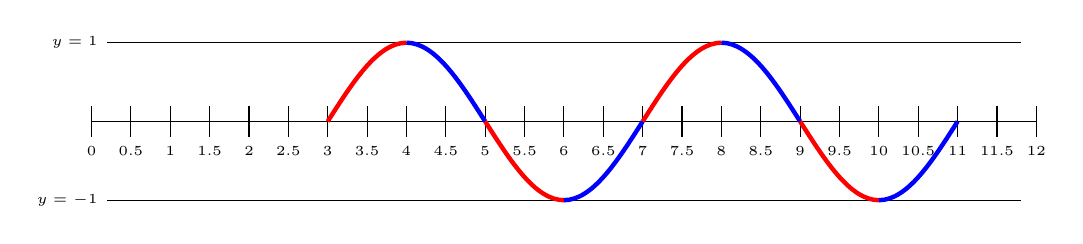
\begin{tikzpicture}

    \draw (0,0) -- (12,0);
    \draw (0.2,1)node[left,font=\tiny] {$y=1$} -- (11.8,1);
    \draw (0.2,-1)node[left,font=\tiny] {$y=-1$} -- (11.8,-1); 
    \foreach \x in {0,0.5,...,12}{
    \draw (\x,-0.2)node [below,font=\tiny,] {\x} -- (\x,0.2) ;
    }
    \draw[ultra thick, red] (3,0) sin (4,1);    %% the real business in this line
    \draw[ultra thick, blue] (4,1) cos (5,0);    %% the real business in this line
    \draw[ultra thick, red] (5,0) sin (6,-1);    %% the real business in this line
    \draw[ultra thick, blue] (6,-1) cos (7,0);    %% the real business in this line
    \draw[ultra thick, red] (7,0)  sin (8,1);    %% the real business in this line
    \draw[ultra thick, blue] (8,1) cos (9,0);    %% the real business in this line
    \draw[ultra thick, red] (9,0) sin (10,-1);    %% the real business in this line
    \draw[ultra thick, blue] (10,-1) cos (11,0);    %% the real business in this line
\end{tikzpicture}
	\caption{Veranschaulichung der Stehenden Welle im Resonanzrohr mit Wellenparametern}
	\label{ab:auswertung->Wellenlaenge->begruendung}
\end{abbildung}
Aus der Abbildung lässt sich folgender Zusammenhang ableiten:
\begin{align}
\label{eq:auswertung->Wellenlaenge->berechnungvorschrift}
\lambda_n &= \frac{\Delta l_n}{n-1}\cdot 2
\end{align}
Mit den Mittelwerten der vier Messungen aus Abschnitt \ref{sub:auswertung->MittelwertResonanzabstand} und der Gleichung \ref{eq:auswertung->Wellenlaenge->berechnungvorschrift} wurde jeweils die Wellenlänge $\lambda$ berechnet und in Tabelle \ref{tab:auswertung->Wellenlaenge->Ergebnis} dargestellt.
\begin{tabelle}
	\caption{Berechnete Wellenlänge für die vier Messungen}
	\label{tab:auswertung->Wellenlaenge->Ergebnis}
	\sisetup{round-precision=2}
	\begin{tabular}{|c|c|c|c|}
		\hline \rowcolor{firstcsvrow}
		Messung & $\overline{\Delta l_n}$ in $cm$ & $n$ & $\lambda$ in $cm$ \\
		\csvreader[separator=semicolon, late after line = \\\hline]{./tables/Ergebnisse.csv}{}
			{\csvcoli~$(\csvcolii~Hz)$ & $\num{\csvcolvi}$ & $\csvcolv$ & $\num{\csvcolvii}$}
	\end{tabular}
\end{tabelle}

\subsection{Berechnung der Schallgeschwindigkeit $c$}
\label{sub:auswertung->Schallgeschwindigkeit}
Die Schallgeschwindigkeit $c$ wurde wie folgt berechnet und ist in Tabelle \ref{tab:auswertung->Schallgeschwindigkeit->Ergebnis} für jede Messung dargestellt.
\begin{align}
c_n&=f_n \cdot \lambda
\end{align}

\begin{tabelle}
	\caption{Ergebnisse der Berechnung der Schallgeschwindigkeit}
	\label{tab:auswertung->Schallgeschwindigkeit->Ergebnis}
	\sisetup{round-precision=1}
	\begin{tabular}{|c|c|c|c|}
		\hline \rowcolor{firstcsvrow}
		Messung & $f$ in $Hz$ & $\lambda$ in $cm$ & $c$ in $m/s$\\
		\csvreader[separator=semicolon, late after line = \\\hline]{./tables/Ergebnisse.csv}{}
			{\csvcoli & $\csvcolii$ & $\num{\csvcolvii}$ & $\num{\csvcolviii}$}
	\end{tabular}
\end{tabelle}

\subsection{Berücksichtigung des Temperatureinflusses}
\label{sub:auswertung->Temperatur}
Die Schallgeschwindigkeiten bei $20~\grad C$ der vier Messungen wurde mit Gleichung (11) berechnet und sind in Tabelle \ref{tab:auswertung->Temperatur->Ergebnis} 

\begin{tabelle}
	\caption{Werte der Schallgeschwindigkeit bei $20~\grad C$ der einzelnen Messungen}
	\label{tab:auswertung->Temperatur->Ergebnis}
	\sisetup{round-precision=2}
	\begin{tabular}{|c|c|c|c|c|}
		\hline \rowcolor{firstcsvrow}
		Messung &  $T_v$ in $\grad C$ & $T_n$ in $\grad C$ & $c$ in $m/s$ & $c_{exp}(20~\grad C)$ in $m/s$\\
		\csvreader[separator=semicolon, late after line = \\\hline]{./tables/Ergebnisse.csv}{}
			{\csvcoli~$(\csvcolii~Hz)$ & $\num[round-precision=1]{\csvcoliii}$ & $\num[round-precision=1]{\csvcoliv}$ & $\num{\csvcolviii}$ & $\num{\csvcolix}$}
	\end{tabular}
\end{tabelle}

\subsection{Zusammenfassung der Ergebnisse und Vergleich mit Literaturwert}
\label{sub:auswertung->Zusammenfassung}
Tabelle \ref{tab:auswertung->zusammenfassung->vergleich} zeigt den Vergleich des experimentellen Wertes $c_{exp}$ mit dem Literaturwert $c_{lit}=\num{343,14}$ in Luft bei $20 ~\grad C$.
\begin{tabelle}
	\caption{Vergleich der Messwerte mit dem Literaturwert bei 20 $\grad C$}
	\label{tab:auswertung->zusammenfassung->vergleich}
	\sisetup{round-precision=3}
	\begin{tabular}{|c|c|c|c|c|}
		\hline \rowcolor{firstcsvrow}
		Messung & $c_{exp}(20~\grad C)$ & $c_{lit}(20~\grad C)$ & abs. Abweichung & rel. Abweichung\\
		\csvreader[separator=semicolon, late after line = \\\hline]{./tables/Ergebnisse.csv}{}
			{\csvcoli~$(\csvcolii~Hz)$ & $\num{\csvcolix}~m/s$ & $\num[round-precision=2]{\csvcolx}~m/s$ & $\num{\csvcolxi}~m/s$ & $\num{\csvcolxii} ~\%$}
		Mittelwert& $\num{333,7448981}~m/s$	& $\num[round-precision=2]{343,14}~m/s$	& $\num{-9,395101917}~m/s$	& $\num{-2,737979226}~\%$
		\\\hline
	\end{tabular}
\end{tabelle}

\subsection{Diskussion der Ergebnisse}
\label{sub:auswertung->Diskussion}
<<<<<<< HEAD
Betrachtet man Tabelle \ref{tab:auswertung->zusammenfassung->vergleich} fällt auf, dass mit steigender Frequenz die Abweichung vom Literaturwert größer wird. Dies liegt wahrscheinlich an der Bandbreite der einzelnen Resonanzfrequenz geringer wird, weil mehr Resonanzen auf der Länge des Resonanzrohres zu messen waren, und somit die Wellenbäuche spitzer und schmaler werden. Daher war Stelle der Auslenkungsmaxima präziser abzulesen. \\
Die sehr geringe Abweichung bei der vierten Messung sieht schön aus, ist allerdings aber mit Vorsicht zu betrachten, d \\
Ein weiterer Grund für Fehler trat beim Ablesen auf. Hier war es schwierig Werte für $l_{max}$ genau zu bestimmen, da man nicht direkt im rechten Winkel auf den Maßstab schauen konnte, sondern, weil das mit Wasser gefüllte Rohr im Weg war, von schräg oben ablesen musste. Dabei schätzen wir eine Messungenauigkeit von $1-2~mm$. \\
%========Marius=================
%Nur eins von beiden sollte übernommen werden
In der Tabelle \ref{tab:auswertung->zusammenfassung->vergleich} kann man sehen, dass die Werte für $c_{exp}(20 ~\grad C)$ mit steigender Frequenz näher am Literaturwert liegen. Dies liegt an der Wellenlänge der stehenden Welle.
Da bei steigender Frequenz die Wellenlänge kleiner wird \ref{tab:auswertung->Wellenlaenge->Ergebnis} und somit die Wellenflanken steiler werden, kann man die Position der Resonanzen besser ablesen.
Da die Wellenflanken bei $500 ~Hz$ sehr flach sind, ist der Fehler dort besonders groß.
Ein weiterer Fehler ergibt sich aus der Ableseungenauigkeit  bei $l_{max}$.
Wenn man $l_{max}$ abgelesen hat, musste man von schräg oben auf die Skala schauen.
Durch die Oberflächenspannung und Lichtbrechung im Wasser schätzen wir einen Parallaxenfehler von $1-2 ~mm$.
=======
Betrachtet man Tabelle \ref{tab:auswertung->zusammenfassung->vergleich} fällt auf, dass mit steigender Frequenz die Abweichung vom Literaturwert größer wird. Dies liegt wahrscheinlich daran, dass die Bandbreite der einzelnen Resonanzfrequenz geringer wird, weil mehr Resonanzen auf der Länge des Resonanzrohres zu messen sind, und somit die Wellenbäuche spitzer und schmaler werden. Daher war die Stelle der Auslenkungsmaxima präziser abzulesen. \\
%Die sehr geringe Abweichung bei der vierten Messung sieht schön aus, ist allerdings aber mit Vorsicht zu betrachten, da  \\
Ein weiterer Grund für Fehler trat beim Ablesen auf. Hier war es schwierig Werte für $l_{max}$ genau zu bestimmen, da man nicht direkt im rechten Winkel auf den Maßstab schauen konnte, sondern von schräg oben ablesen musste, weil das mit Wasser gefüllte Rohr im Weg war. Dabei schätzen wir eine Messungenauigkeit von $1-2~mm$. 
Für die Messung wäre auch eine ausführliche Fehlerrechnung möglich, um so die Ergebnisse besser zu beurteilen.
%========Marius=================
>>>>>>> 11383cb15528263684be821ce85c924a678ec7c6
